%==============================%
%  D o c u m e n t  S t y l e  %
%==============================%
\documentclass[enabledeprecatedfontcommands,parskip=half,twoside=semi,BCOR=0mm]{scrreprt}
%,bibliography=totoc


\usepackage[utf8]{inputenc}
\usepackage[T1]{fontenc}
\usepackage{lmodern}
\usepackage[english,ngerman]{babel}
\usepackage{subfig}
\usepackage{amssymb}

\usepackage{wallpaper}

\usepackage{float} %for graphics positioning
%\usepackage{subfigure} %for two figures next to each other

\usepackage{csquotes}
\usepackage[backend=biber, style=authoryear]{biblatex}
\addbibresource{bibliopaper.bib} % with extension
\setlength{\bibitemsep}{1.5\baselineskip}
\setlength{\parindent}{0pt}
\newcommand{\tab}[1]{\hspace{.2667\textwidth}\rlap{#1}}
\newcommand{\itab}[1]{\hspace{0em}\rlap{#1}}
 
%=====================%
%  M a t h e z e u g  %
%=====================%
\usepackage[hidelinks]{hyperref}    %Referenzen ohne Kästchen im pdf
\usepackage{amsmath,amsthm,amssymb} %Mathe-stuff
\usepackage{mathtools}
\usepackage{microtype}              %hübscheres Spacing etc

\usepackage{graphicx}
\usepackage{amsmath}
\usepackage{mathtools}
\usepackage{bm}
\usepackage{adjustbox}

\usepackage{tabularx} % schöne Tabellen
\newcolumntype{L}[1]{>{\raggedright\arraybackslash}p{#1}} % linksbündig mit Breitenangabe
\newcolumntype{C}[1]{>{\centering\arraybackslash}p{#1}} % zentriert mit Breitenangabe
\newcolumntype{R}[1]{>{\raggedleft\arraybackslash}p{#1}}

\mathtoolsset{centercolon}
 \parindent0pt

\mathtoolsset{centercolon}

\DeclarePairedDelimiter\floor{\lfloor}{\rfloor}
\DeclarePairedDelimiter\ceil{\lceil}{\rceil}

\addtokomafont{disposition}{\rmfamily} %serifen in jedem Titel 


\numberwithin{equation}{chapter}
\newtheorem{theorem}{Theorem}[chapter] %amsthm-stuff
\newtheorem{proposition}[theorem]{Proposition}
\newtheorem{lemma}[theorem]{Lemma}
\newtheorem{corollary}[theorem]{Corollary}

\theoremstyle{definition}
\newtheorem{definition}[theorem]{Definition}
\newtheorem{remark}[theorem]{Remark}
\newtheorem{assumption}{Assumption}
\newtheorem{example}[theorem]{Example}

\theoremstyle{remark}
\newtheorem*{claim}{Claim}

%=====================%
%  S o n s t i g e s  %
%=====================%
\usepackage{comment} % auskommentieren ganzer Zei
\usepackage[ruled,vlined]{algorithm2e}  % Pseodo-Code

% TODO Package Style
\usepackage{lipsum}                     % Dummytext
\usepackage{xargs}                      % Use more than one optional parameter in a new commands
\usepackage{xcolor}  % Coloured text etc. [pdftex,dvipsnames]
\usepackage[colorinlistoftodos,prependcaption,textsize=tiny]{todonotes}
\newcommandx{\unsure}[2][1=]{\todo[linecolor=red,backgroundcolor=red!25,bordercolor=red,#1]{#2}}
\newcommandx{\change}[2][1=]{\todo[linecolor=blue,backgroundcolor=blue!25,bordercolor=blue,#1]{#2}}
\newcommandx{\info}[2][1=]{\todo[linecolor=purple,backgroundcolor=purple!25,bordercolor=purple,#1]{#2}}
\newcommandx{\improvement}[2][1=]{\todo[linecolor=green,backgroundcolor=green!25,bordercolor=green,#1]{#2}}








%=============%
%  T i t l e  %
%=============%
\pagestyle{headings}
\titlehead{
    \centering Ludwig-Maximilians-Universität München 
    \par Fakultät für Mathematik, Informatik und Statistik
    \par Institut für Statistik}
\subject{SS 24 Seminar\\
Areal Data Analysis}
\title{Areal Wombling}
\author{\\
Name: Sameer Singh Rawat\\
Matriculate number: 12691600\\
PO 2021\\
Master's Statistics and Data Science\\
Module: Advanced Research Methods in Machine Learning}
\date{}
\publishers{Supervisor: Martje Rave}




\begin{document}
    \selectlanguage{english}

	
    % title page
    \ThisTileWallPaper{\paperwidth}{\paperheight}{Siegelwallpaperblank.pdf}
    \maketitle
    
    % content
    \tableofcontents
    %\listoffigures
    %\listoftables
    %\listofalgorithms
	\newpage
    
    \chapter{Introduction}
    Wombling is a technique of identifying edges or boundaries of rapid change. It is often referred to as edge detection or barrier analysis. It has become increasingly popular in the fields of environmental sciences and public health. Wombling can further be classified into two types - crisp and fuzzy wombling. In crisp wombling we assume that boundaries obtained are sharp and clear, identifying the regions of significant change while in fuzzy wombling the boundaries are assumed to be unclear and fuzzy with the goal of understanding gradual change in attribute values.
    
    \section{Motivation}
    The motivation behind this project stems from the importance of understanding and quantifying abrupt change in variables of interest such as drastic change in disease rate or ecological variables across regions.
    
    In context of covid-19 pandemic, precisely detecting these boundaries of significant change can help us identify areas where the policies and medical services were not able to tackle covid cases. These results not only in covid scenario but also at general level can help us improve the healthcare system and policies of regions, and thus of whole country.  
    
    \section{Literature review}
    The concept of wombling was first established by statistician named William H. Womble in the year 1951. Since then over many years, there has been many advancements in its methods and applications. In their paper Ecological boundary detection using Bayesian areal wombling, \cite{Fitzpatrick.2010} have used Bayesian hierarchical modelling framework in context of fuzzy areal wombling for detecting and assigning probabilities to boundaries. They have focused on hierarchical wombling approach and stated that it is better than the classical approaches which do not account for spatial structure and uncertainty in data.They have used this setting in analyzing ecological boundaries to account for how the distribution of species, hemlock woolly adelgid (Adelges tsugae) change across US counties and has also taken into account the possible covariates affecting this change.

    In another paper, \cite{Lu_Carlin.2005} proposed a model based approach for detecting boundaries using Bayesian hierarchical framework. They highlight the challenges associated with areal data which is often aggregated over a large area due to confidentiality and data collection constraints. In this paper they explore both the traditional algorithm and Bayesian approach and again show how Bayesian methods have improved accuracy by accounting for spatial dependence and covariates. Their framework also takes into account crisp and fuzzy wombling approaches.
        
    Both these paper highlights the evolution of simplistic traditional algorithms to more sophisticated modelling based approaches, the latter outperforming the former by taking into account the spatial and statistical complexities. In this seminar paper we will see how these both techniques in context of crisp areal wombling, can be applied to covid-19 data. We would be focusing on Standardized Death Rate (SDR) across states of US during the month of April 2020. The goal of this study is to compare both the traditional and modelling based approach and identify the regions with significant difference in SDRs, which can highlight the potential regions for improving healthcare responses.

    \chapter{Data}
    For the study of covid-19 cases we have taken the data for the time period of April 2020. The selection of year 2020 was based on the fact that it was the year when the first surge in the number of covid cases were encountered and more specifically it was in the month of April when there was a first major spike in the number of covid cases in the US.  
    
    The major component that we needed for our study was Standardized Death Rate (SDR), for the calculation of this we needed the number of deaths and also the number of confirmed covid cases. Data for both these values for the time period of April 2020 were taken from the github repository of Center for Systems Science and Engineering (\cite{CSSE}), John Hopkins University. 
    
    For performing, Bayesian  hierarchical modelling we needed some covariates. There could have been many possible covariates affecting the SDR (i.e. the deaths and confirmed covid cases) but we have taken number of Hospital beds per 1000 people and proportion of people above the age of year 65 as our covariates. It is quite obvious that number of hospital beds and the population of old people in a state are genuine covariates. But the number of hospital beds per 1000 people and  proportion of older people is taken so that we can standardize our study and account for different population in different states. Also another point to note here is that since the data for the covariates was available for the year as a whole i.e. either for 2019 or 2020, here we have taken the data from 2019. It is just to mitigate any bias that might arise from the measures or demographic change that might have took place after April 2020, since if we take the data of 2020 it would reflect changes in covariate values that might have changed drastically after April 2020 (after which the serious measures were taken in most of the countries). Having said that some, although different type of information loss will still be there while taking the data for year 2019, since in this we are ignoring the measures that have been taken by the state government from Jan 2020 to March 2020 to tackle covid-19, but if we want to make conclusions about the general healthcare policies and infrastructure, we should be fine with taking data from the year 2019. The data for our covariates was taken from the Kaiser Family Foundation (\cite{KFF}) website.

    The shapefiles for US states is taken from US Census Bureau website (\cite{USBC}).
    \chapter{Methodology}
    In this section we will discuss how we went about performing our study in mathematical detail. 

    \section{Standardized Death Rate (SDR)}
    Firstly, we see how our variable of interest - SDR is calculated?
    Our primary variable of interest is the proportion of deaths to the confirmed cases reported due to covid-19. The reason why this serves as our variable of interest is, because it shows, given the certain number of covid cases how the health care infrastructure and governance were able prevent the deaths. This is what SDR basically implies. The lower proportion of this number means healthcare system was robust in tackling covid cases.
    The Standardized Death Rate (SDR) for region \(i\) is given by:
    \[
    \text{SDR}_i = \frac{Y_i}{E_i} \quad \text{for } i = 1, 2, \ldots, N
    \]
    where:
    \begin{itemize}
        \item \(Y_i\) is the observed number of deaths in region \(i\),
        \item \(E_i\) is the expected number of deaths in region \(i\), and
        \item \(N\) is total number of regions/states (in our case 51)
    \end{itemize}

    The expected number of deaths \(E_i\) in region \(i\) is calculated as:
    \[
    E_i = n_i \times \bar{r}
    \]
    \[
    \bar{r} = \frac{\sum_{i=1}^{n} Y_i}{\sum_{i=1}^{n} n_i}
    \]
    where, \(n_i\) is number of confirmed cases in ith state.
    
    \section{Spatial Auto correlation}
    
    The first step towards analysis of data is to simply measure spatial auto correlation among the values of SDRs with the help of Moran I test statistic. Spatial auto correlation measures the degree to which values at nearby locations are similar or dissimilar to each other. Positive spatial auto correlation means similar values are clustered together in space while negative spatial auto correlation means dissimilar values are clustered together in space. 
    
    The moran I test statistic for our case is moderately positive with the value of 0.28 and is statistically significant at 5\% level of significance with p-value of 0.001. We also plot moran scatterplot (see Figure \ref{fig:Figure 1}) and see the upward sloping line which again confirms that our spatial auto correlation is positive. It is easy to understand moran scatterplot. In the x axis is the standardized values of SDR and in y axis is the spatial lag of standardized SDR (note, that the negative value on both the axes is due to standardization). The spatial lag is the average of the variable in its neighbouring regions. For example, spatial lag of standardized SDR at A = average value of standardized SDRs at neighbouring regions of A. Hence if the real value of the standardized SDRs at states is same as the average value of standardized SDRs at their respective neighbouring states then we can see an upward sloping line. Hence, a positive spatial auto correlation. This shows that states with similar SDRs are likely to be present close to each other.
    \begin{figure}[h]
    \centering
    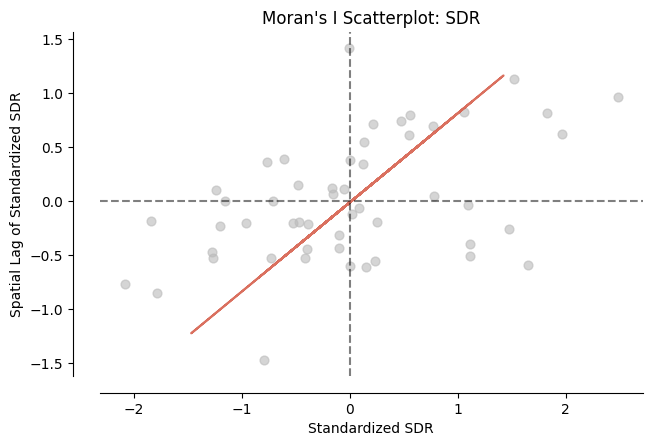
\includegraphics[width=0.75\textwidth]{Moran_I.png}
    \caption{Moran scatter plot}
    \label{fig:Figure 1}
    \end{figure}
    
    \section{Plotting of SDRs}
    
    For visualizing our data we can simply plot the heatmap of SDRs of the states and see how SDRs change over the US states. Here we can begin to speculate where there is drastic change in SDR values and thus where boundaries would likely be generated. (See Figure \ref{fig:Figure 2})
    \begin{figure}[h]
    \centering
    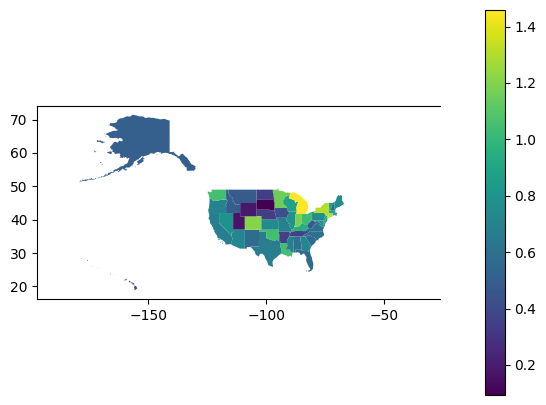
\includegraphics[width=0.75\textwidth]{SDR.png}
    \caption{SDR Heatmap}
    \label{fig:Figure 2}
    \end{figure}
    
    \section{Traditional Crisp Wombling}
    
    This a simplistic approach and no modelling is necessary in this approach. In this we simply take a state and calculate the difference of its SDR value with SDRs of each of its neighbouring states, and call it the Boundary Likelihood Value (BLV) for that pair of states. For example, suppose we have a state A and its neighbours are B and C. Then the BLVs of (A,B) and (A,C) are \(|SDR(A)-SDR(B)|\) and \(|SDR(A)-SDR(C)|\) respectively. Then we calculate our threshold. Since there is no concrete way to calculate the threshold in the researches, we have followed the approach of \cite{Lu_Carlin.2005}, and calculated two thresholds, one by taking 50 percentile value of BLVs and second by taking 80 percentile value of BLVs. And then we mark the boundaries by blue between the neighbouring states where BLV for that pair of states is greater than 50 percentile and with red if the BLV for that pair of states is greater than 80 percentile.

    The boundaries that we have obtained by this method can be seen in Figure \ref{fig:Figure 3}
    \begin{figure}[h]
    \centering
    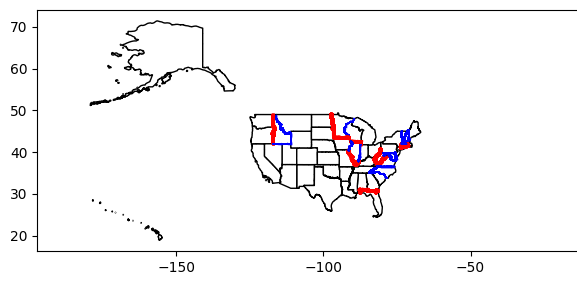
\includegraphics[width=0.75\textwidth]{Traditional.png}
    \caption{Traditional Wombling}
    \label{fig:Figure 3}
    \end{figure}
    
    \section{Hierarchical modelling approach}
    
    In this we will try to account for the weakness of the traditional wombling method by incorporating for the variability and spatial correlation in response variable Y (i.e number of deaths, in our case).
    
    As per the researches, as highlighted by \cite{Lu_Carlin.2005}, for count data the most suited way to model our response variable is by Poison log linear form.
    
    \[ Y_i \sim \text{Poisson}(\mu_i) \]
    where,
    \[
    \log(\mu_i) = \log(E_i) + \mathbf{x}_i^T \beta + \phi_i
    \]
    
    Here our \(X_i\)'s denote our covariates - Hospital beds per 1000 people and proportion of people aged above 65, while \(\beta_1\) and \(\beta_2\) denote their respective coefficients. The prior for \(\beta_1\) and \(\beta_2\) that we have taken in the model are normal distribution with mean 0 and standard deviation 10.
    
    Also for modelling random effects \(\phi_i\)'s we have used a form of Conditional Auto regressive model called Intrinsic Conditional Auto regressive model (ICAR). The ICAR assumes that the random effect for a particular region is influenced by the effects of neighbouring regions as specified by the adjacency matrix (in our case we have taken Queen Contiguity Adjacency Matrix). The ICAR model have the conditional distribution of the form:
    \[
    \phi_i \mid \phi_j \text{ for } j \neq i \sim \mathcal{N}\left(\bar{\phi_i}, \frac{1}{\tau \cdot m_i}\right)
    \]

    where,
    \(\bar{\phi}_i\) is average of \(\phi_{j \neq i}\) that are adjacent to \(\phi_i\) and \(m_i\) is the number of neighbours of ith state while \(\tau\) is set to some constant number.
    
    With these model specifications we run Markov chain Monte Carlo (MCMC) algorithm with 2 chains to get 1000 samples for \(\mu\) after tuning for 1000 iterations. For this we use pymc package in python. 
    
    After running our MCMC algorithm we plot the trace plots for each of the parameters \(\beta_1\), \(\beta_2\) and \(\phi\)'s
    \begin{figure}[h]
    \centering
    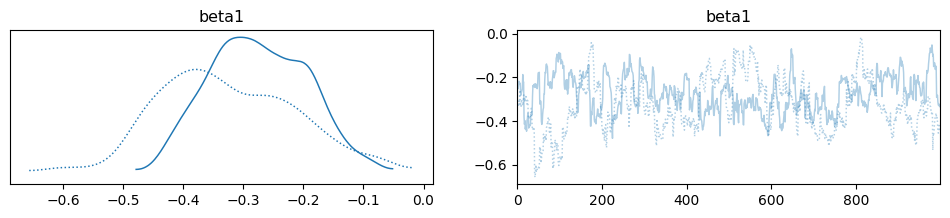
\includegraphics[width=0.75\textwidth]{traceplot_beta1.png}
    \caption{Trace plot \(\beta_1\)}
    \label{fig:Figure 4}
    \end{figure}
    \begin{figure}[h]
    \centering
    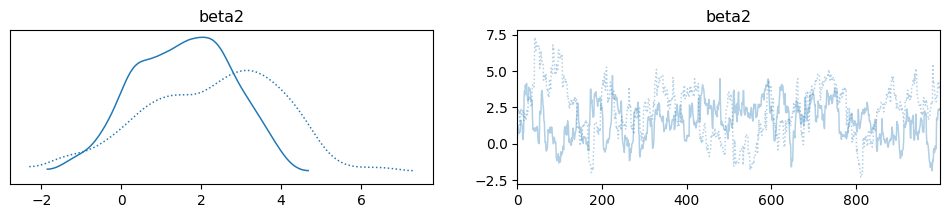
\includegraphics[width=0.75\textwidth]{traceplot_beta2.png}
    \caption{Trace plot \(\beta_2\)}
    \label{fig:Figure 5}
    \end{figure}
    \begin{figure}[h]
    \centering
    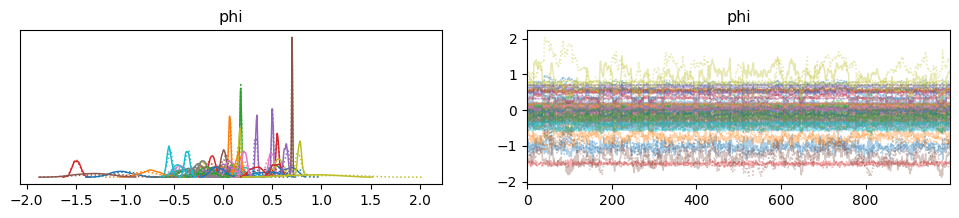
\includegraphics[width=0.75\textwidth]{traceplot_phi.png}
    \caption{Trace plot \(\phi\)'s}
    \label{fig:Figure 6}
    \end{figure}

    From the trace plots we can see that the MCMC algorithm has somewhat converged since the plot is oscillating around a point and also the two chains somewhat overlap over each other showing that the samples in both chains come from the same distribution.

    To further confirm the convergence of MCMC algorithm we can find gelman rubin statistic (r-hat) values for each of the parameter and see that for each of the parameter it is below 1.1 (See Table \ref{tab:Table 1}).
    \begin{table}[h!]
    \centering
    \begin{adjustbox}{max width=\textwidth}
    \begin{minipage}{0.48\textwidth}
    \centering
    \begin{tabular}{l r}
    \textbf{Parameter} & \textbf{r\_hat} \\
    \hline
    beta1 & 1.05 \\
    beta2 & 1.05 \\
    phi[0] & 1.02 \\
    phi[1] & 1.05 \\
    phi[2] & 1.01 \\
    phi[3] & 1.01 \\
    phi[4] & 1.05 \\
    phi[5] & 1.05 \\
    phi[6] & 1.04 \\
    phi[7] & 1.04 \\
    phi[8] & 1.04 \\
    phi[9] & 1.04 \\
    phi[10] & 1.05 \\
    phi[11] & 1.05 \\
    phi[12] & 1.04 \\
    phi[13] & 1.05 \\
    phi[14] & 1.04 \\
    phi[15] & 1.05 \\
    phi[16] & 1.05 \\
    phi[17] & 1.05 \\
    phi[18] & 1.04 \\
    phi[19] & 1.05 \\
    phi[20] & 1.05 \\
    phi[21] & 1.03 \\
    phi[22] & 1.04 \\
    \end{tabular}
    \end{minipage}
    \hfill
    \begin{minipage}{0.48\textwidth}
    \centering
    \begin{tabular}{l r}
    \textbf{Parameter} & \textbf{r\_hat} \\
    \hline
    phi[23] & 1.00 \\
    phi[24] & 1.01 \\
    phi[25] & 1.04 \\
    phi[26] & 1.04 \\
    phi[27] & 1.04 \\
    phi[28] & 1.04 \\
    phi[29] & 1.02 \\
    phi[30] & 1.02 \\
    phi[31] & 1.04 \\
    phi[32] & 1.04 \\
    phi[33] & 1.05 \\
    phi[34] & 1.04 \\
    phi[35] & 1.01 \\
    phi[36] & 1.05 \\
    phi[37] & 1.01 \\
    phi[38] & 1.05 \\
    phi[39] & 1.03 \\
    phi[40] & 1.05 \\
    phi[41] & 1.04 \\
    phi[42] & 1.01 \\
    phi[43] & 1.04 \\
    phi[44] & 1.04 \\
    phi[45] & 1.04 \\
    phi[46] & 1.04 \\
    phi[47] & 1.05 \\
    phi[48] & 1.05 \\
    phi[49] & 1.01 \\
    phi[50] & 1.05 \\
    \end{tabular}
    \end{minipage}
    \end{adjustbox}
    \caption{Parameters and their corresponding r\_hat values}
    \label{tab:Table 1}
    \end{table}

    
    
    In python we did not get samples for \(\mu_i\)'s directly in the result, but we got samples of \(\beta_1\), \(\beta_2\) and \(\phi\)'s. And we calculated \(\mu_i\)'s by using the equation 
    \[
    \mu_i = \exp(\log(E_i) + \mathbf{x}_i^T \beta + \phi_i)
    \] 
    
    Hence, we get 1000 samples of \(\mu\) with each sample having 51 values(equal to number of states in our dataset). 
    
    Now to calculate SDR we use the formula 
    \[
    Z_i = \frac{\mu_i}{E_i} \quad \text{for } i = 1, 2, \ldots, 51
    \]
    and transform this into a matrix with 1000 rows and 51 columns with each column representing a state and each row one of the samples generated from MCMC algorithm. So Z can be thought of a matrix of dimension \(1000\times51\). 
    
    Now to calculate Boundary likelihood values we use the formula
    \(D_{ij}\)=\(|Z_i-Z_j|\) for all i adjacent to j where \(Z_i\) and \(Z_j\) represent the ith column and jth column (or more precisely ith and jth state) of the Z matrix respectively. Since each of the column contains 1000 values so their difference \(D_{ij}\) will also have 1000 values. Thus we can calculate 
    \[
    \mathbb{E}(D_{ij} \mid y) = \frac{1}{1000} \sum_{g=1}^{1000} D_{ij}^{(g)}
    \]
    which, gives us the boundary likelihood value for each pair of states i and j.
    
    Again we use \cite{Lu_Carlin.2005} methodology to calculate the thresholds by computing the 50 percentile and 80 percentile of BLVs and mark the boundaries of the states whose boundary likelihood values exceed these thresholds by blue and red colour respectively.

    The plot we obtained by this method can be seen in the Figure \ref{fig:Figure 7}
    \begin{figure}[h]
    \centering
    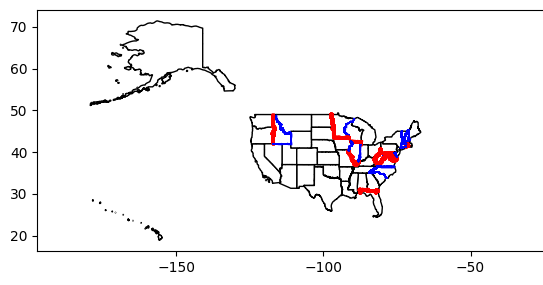
\includegraphics[width=0.75\textwidth]{Hierarchical.png}
    \caption{Hierarchical Modelling Approach}
    \label{fig:Figure 7}
    \end{figure}

    \chapter{Results}
    Firstly we can very clearly see from moran I test statistic and moran scatterplot that our data i.e. SDR values have spatially positive auto correlation. Hence, stating that places with similar values of SDR are close to each other. Thus it clearly shows us the scope to perform spatial analysis with our data. 
    
    Now we can compare the plots (see Figure \ref{fig:first} and Figure \ref{fig:second}) that we got from both traditional and hierarchical modelling approach. Here we can see that traditional method fails to capture some of the boundaries that were captured by hierarchical modelling that took into account the variability and spatial correlation of our observed variable SDR or more specifically deaths.
   
    \begin{figure}[h!]
        \centering
        % First image
        \begin{minipage}[b]{0.45\textwidth}
            \centering
            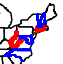
\includegraphics[width=\textwidth]{Traditional_copy.png}
            \caption{Traditional Approach}
            \label{fig:first}
        \end{minipage}
        \hfill
        % Second image
        \begin{minipage}[b]{0.45\textwidth}
            \centering
            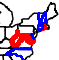
\includegraphics[width=\textwidth]{Hierarchical - Copy.png}
            \caption{Hierarchical modelling Approach}
            \label{fig:second}
        \end{minipage}
    \end{figure}
        
    
    Finally on the basis of the results derived from hierarchical modelling approach (See Table \ref{tab:boundary_diff})  we can conclude that the states of Minnesota, Colorado, Louisiana, Oklahoma, Michigan, Nevada, Kentucky, New York, Arizona, Washington, Connecticut, Ohio are the states where the deaths to confirmed cases ratio is significantly higher than their neighbouring states, hence signifying probable scope of improvement in healthcare facilities.
    \begin{table}[h!]
    \centering
    \begin{adjustbox}{max width=\textwidth}
    \begin{tabular}{|l|l|c|c|c|c|}
        \hline
        \textbf{State1} & \textbf{State2} & \textbf{boundary\_diff} & \textbf{significant\_20} & \textbf{significant\_50} & \textbf{greater\_SDR} \\
        \hline
        Minnesota & South Dakota & 1.058422 & True & True & Minnesota \\
        Utah & Colorado & 1.042243 & True & True & Colorado \\
        Colorado & Wyoming & 1.019429 & True & True & Colorado \\
        Nebraska & Colorado & 0.873460 & True & True & Colorado \\
        Minnesota & North Dakota & 0.820936 & True & True & Minnesota \\
        Minnesota & Iowa & 0.726403 & True & True & Minnesota \\
        Louisiana & Arkansas & 0.700580 & True & True & Louisiana \\
        Oklahoma & Arkansas & 0.694566 & True & True & Oklahoma \\
        Illinois & Michigan & 0.677412 & True & True & Michigan \\
        New Mexico & Colorado & 0.637753 & True & True & Colorado \\
        Utah & Nevada & 0.619279 & True & True & Nevada \\
        Tennessee & Kentucky & 0.593245 & True & True & Kentucky \\
        Rhode Island & New York & 0.590660 & True & True & New York \\
        Wisconsin & Michigan & 0.576070 & True & True & Michigan \\
        Utah & Arizona & 0.553806 & True & True & Arizona \\
        Idaho & Washington & 0.549143 & True & True & Washington \\
        Pennsylvania & New York & 0.547768 & True & True & New York \\
        Rhode Island & Connecticut & 0.547252 & True & True & Connecticut \\
        West Virginia & Ohio & 0.545112 & True & True & Ohio \\
        Colorado & Arizona & 0.488437 & True & True & Colorado \\
        New Mexico & Oklahoma & 0.470177 & True & True & Oklahoma \\
        West Virginia & Kentucky & 0.463428 & True & True & Kentucky \\
        Colorado & Kansas & 0.457913 & True & True & Colorado \\
        \hline
    \end{tabular}
    \end{adjustbox}
    \caption{Boundary Likelihood Values (BLVs) between states from highest to lowest based on Hierarchical Approach}
    \label{tab:boundary_diff}
    \end{table}

    \chapter{Conclusion and Discussion}
    In this seminar paper we have explored the concept of wombling in detail keeping it simple to understand and implement. This paper can give us some intuition on how wombling can be used to analyze the healthcare situations over a given region using areal data. Such analysis can help us focus on the areas which were not able to perform well to tackle the spread of some disease and help us take some measures to counter this. This seminar paper is unique from most of the research papers that have already been published in the field of wombling in a way that it implements the whole spatial analysis in python rather than R, latter being more popular language in the field of spatial analysis. Most of the parameters and model specifications are similar to the ones used by \cite{Lu_Carlin.2005} in their paper. This paper too like many research papers in the past establishes the superiority of hierarchical approach over traditional approach when performing wombling.
    
    Having said that this paper shows us how one can perform sophisticated technique like wombling in a simple and easy to understand manner, there are some limitations. Firstly, when we performed the t-test between the Boundary Likelihood values that were generated from our traditional approach and hierarchical approach we did not find those samples to be statistically different. This can be an indication that Hierarchical modelling cannot always be proved to be significantly better than traditional approach. When researching about what could have gone wrong, one of the most obvious reason that seems, is the choice of the prior distribution of betas or maybe our failure to account for some important covariates during modelling. Another shortcoming that we faced was while running the code in python some of the instances of code (like running MCMC algorithm) took too much time. Also, since these analysis are done at state level, we might need to do post hoc analysis at district levels of each states to better know about the situations at a finer level. 
    
    There is also another thing to note, that since in our analysis we have done crisp wombling, we assume that changes in SDRs between states are significant and quick, and there are clear boundaries between the states with different SDRs. We can extend this analysis by performing fuzzy wombling again by traditional and hierarchical approach. In fuzzy wombling we assume that the changes of variable of interest is gradual which might result in unclear and fuzzy boundaries. The difference in methodology is that instead of assigning the boundary in a discrete manner such that if the BLVs exceed some threshold value c, we now assign probability to the boundary by calculating \(p_{ij}\)(\(D_{ij}\)>c/y) which is equal to \#(\(D_{ij}\)>c)/G where G is the number of draws from MCMC algorithm.

   \appendix
    \chapter{GitHub Repository}
    The complete source code and additional materials can be found at \href{https://github.com/SameerR007/ArealWombling_Project}{GitHub Repository (click here).}
    
    % Bibliographie
    \newpage
    \addcontentsline{toc}{chapter}{Bibliography}
    \printbibliography

\end{document}
